\documentclass[12pt,a4paper]{article}
\usepackage[latin1]{inputenc}
\usepackage{amsmath,bm}
\usepackage{amsfonts}
\usepackage{amssymb}
\usepackage{makeidx}
\usepackage{graphicx}
\usepackage{float}
\usepackage{color}
\usepackage{xcolor}
\usepackage[colorlinks,linkcolor=blue,anchorcolor=blue,citecolor=blue]{hyperref}
\usepackage{amsmath,amsthm,amssymb}

\usepackage[level]{datetime}

%\usepackage{wasysym}
%\usepackage{marvosym}

%\usepackage{ctexcap}

\usepackage{amsmath}
\usepackage{amssymb}
\usepackage{array}
\usepackage{amsmath,subfigure}%,psfig
\usepackage{algorithm}
\usepackage{booktabs}
\usepackage{multirow}
\usepackage{colortbl}
\definecolor{tabcolor}{rgb}{.105,.410,.113}


\usepackage{geometry}
\geometry{left=2.5cm,right=2.5cm,top=2.5cm,bottom=2.5cm}
\linespread{1.25}
%\linespread{1.05}
\setlength{\parskip}{0.5\baselineskip}

\usepackage{lastpage}%获得总页数

%\addtolength{\hoffset}{-1.2cm}%增加左边距-2cm
%\addtolength{\voffset}{-1.5cm}%增加上边距-3cm
%\addtolength{\textwidth}{2.4cm}%增加文本区域宽度4cm
%\addtolength{\textheight}{3cm}%增加文本区域高度5cm


\usepackage[center]{titlesec}
\renewcommand{\thefootnote}{\fnsymbol{footnote}}
\renewcommand{\baselinestretch}{1.1}%{1.2}
\newcommand{\dachu}{\fontsize{48pt}{\baselineskip}\selectfont}
\newcommand{\chuhao}{\fontsize{42pt}{\baselineskip}\selectfont}
\newcommand{\xiaochuhao}{\fontsize{36pt}{\baselineskip}\selectfont}
\newcommand{\yihao}{\fontsize{28pt}{\baselineskip}\selectfont}
\newcommand{\xiaoyihao}{\fontsize{24pt}{\baselineskip}\selectfont}
\newcommand{\erhao}{\fontsize{21pt}{\baselineskip}\selectfont}
\newcommand{\xiaoerhao}{\fontsize{18pt}{\baselineskip}\selectfont}
\newcommand{\sanhao}{\fontsize{15.75pt}{\baselineskip}\selectfont}
\newcommand{\xiaosanhao}{\fontsize{15pt}{\baselineskip}\selectfont}
\newcommand{\sihao}{\fontsize{14pt}{\baselineskip}\selectfont}
\newcommand{\xiaosihaomore}{\fontsize{13pt}{1.12\baselineskip}\selectfont}
\newcommand{\xiaosihao}{\fontsize{12pt}{1.12\baselineskip}\selectfont}
\newcommand{\xiaosihaoless}{\fontsize{12pt}{0.8\baselineskip}\selectfont}
\newcommand{\wuhao}{\fontsize{10.5pt}{\baselineskip}\selectfont}
\newcommand{\xiaowuhao}{\fontsize{9pt}{\baselineskip}\selectfont}
\newcommand{\liuhao}{\fontsize{7.875pt}{\baselineskip}\selectfont}
\newcommand{\qihao}{\fontsize{5.25pt}{\baselineskip}\selectfont}

\renewcommand{\normalsize}{\xiaosihao}%less}

\titleformat{\section}{\sihao\bfseries}{\thesection}{1em}{}
\titleformat{\subsection}{\xiaosihaomore\bfseries}{\thesubsection}{1em}{}
\titleformat{\subsubsection}{\xiaosihaomore\bfseries}{\thesubsubsection}{1em}{}

\title{User Manual of TeXpen}
\author{MengChang Wang}

\newcommand{\upcite}[1]{\textsuperscript{\cite{#1}}}

\newcommand{\texpen}{{\TeX}pen~}

%\newdateformat{ukdate}{\ordinaldate{\THEDAY} \monthname[\THEMONTH] \THEYEAR}%日月年

%\renewcommand{\today}{\number\day, \number\month, \number\year}

\renewcommand{\today}{\number\day,\space\ifcase\month\or
Jan\or Feb\or Mar\or Apr\or May\or Jun\or
Jul\or Aug\or Sep\or Oct\or Nov\or Dec\fi,
\space\number\year}

\usepackage{fancyhdr}
\pagestyle{fancy}
\fancyhf{}
\fancyhead[L]{\color{gray}{ \textit{User Manual of {\TeX}pen }}}%
\includegraphics[width=3.0cm]{figs/texpen.png}}
\fancyhead[R]{
\includegraphics[width=0.8cm]{figs/texpen.png}}%{\empty}%\textit{Survey Report\\$\;$}}
\fancyfoot[R]{\thepage/\pageref{LastPage}}%{Page \thepage/8}
\fancyfoot[L]{\scriptsize\textit{		
		\today %插入当前日期
	}}%School of Mechanical \& Aerospace Engineering}}
\renewcommand{\headrulewidth}{1pt} 
\setlength{\headsep}{0.8cm}


%%%%%%%%%TikZ
\usepackage{pgf}
\usepackage{tikz}
\usetikzlibrary{arrows,automata}
\usetikzlibrary{positioning}
%%%%%%%%%TikZ

\usepackage{fontspec}
%\usepackage{charter}
\usepackage{mathpazo}
%\setmainfont{Liberation Serif}%[BoldFont=SimHei]{Palatino}



\renewcommand{\contentsname}{CONTENTS}
\renewcommand{\refname}{REFERENCES}



%%%%%%%%%%%%%%%%%%%%%%%%%%%%%%%%%%%%%%%%%%%%%
%%%%%%%%%%%%%%%%%%%%%%%%%%%%%%%%%%%%%%%%%%%%%
%%%%%%%%%%%%%%%%%%%%%%%%%%%%%%%%%%%%%%%%%%%%%

\begin{document}

%\maketitle


%%%%%%%%%%%
%% Cover Page %%

%\pagestyle{plain}
\thispagestyle{empty}
$\;$\\

\begin{flushright}
\begin{tabular}{l}
\arrayrulecolor{tabcolor}
\toprule [1pt]
\\
\xiaoerhao {User Manual of {\TeX}pen }\\ [1.2ex]
\\
\hline
$\;$\\ [1.2ex]
\sihao {Dr. WANG MengChang} \\ [1.2ex]
\\
\hline
$\;$\\ [1.2ex]
\wuhao {wangmengchang@gmail.com } \\ [1.2ex]
\\
\bottomrule [1pt]
\end{tabular}
\end{flushright}

\vfill


\begin{picture}(1,1)
\put(-20,-3){
\includegraphics[width=3cm]{figs/texpen.png}}
\end{picture}

%\begin{picture}(1,1)
%\put(300,-2.5){\includegraphics[width=4.8cm]{figs/ntu.png}}
%\end{picture}

%\noindent
%\begin{flushright}
% \includegraphics[height=1.8cm]{figs/ntu.png}\\
%\end{flushright}

\clearpage
\setcounter{page}{1}
\thispagestyle{empty}

$\;$


\vspace{6cm}

%I have a dream, where the computer helps me thinking, but I twinkle the cursor. 
I have a dream, where the computer helps me think, but I twinkle the sparks in my eyes. 

\begin{picture}(1,1)
\put(90,-90){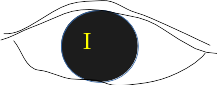
\includegraphics[width=6cm]{figs/eye.png}}
\end{picture}



\clearpage
\setcounter{page}{1}
\pagestyle{fancy}


\tableofcontents
\clearpage
%\listoftables       %表目录
%\clearpage
\listoffigures     %图目录



\clearpage
\setcounter{page}{1}


\section{INTRODUCTION}

{\TeX}pen is an editor started when I was preparing for my manuscript in my days as a PhD student. Later on, it was improved so that my PhD dissertation can be written with it, about 100,000 Chinese characters with all kinds of equations, figures and tables.

{\TeX}pen aims at lessening the burden of scientific writers in preparing articles, slides and books, and it is still in perhaps endless development and improvement. However, just like any of the majority of those open source projects, {\TeX}pen is provided free of charge, free of guarantee, free of promise, and free of restriction, but full of tiny bugs, full of thirsty for donations, and full of desires for feedbacks.


\section{Environment \& Installation}

{\TeX}pen  is an editor, and you can use it to edit any text file, including plain text files, c plus plus source files, and HTML source files among others. However, it would be happier if you use it for \LaTeX editing.

So, you'd better to have a \TeX /\LaTeX ~environment, although \texpen is able to work functionally without it.

\subsection{\TeX/\LaTeX ~Environment}
The \TeX ~is created by the great professor, Knuth, and \LaTeX ~is an great extension on \TeX . 

\subsection{\LaTeX ~Basis}


\subsection{\texpen ~Installation}



\bibliographystyle{ieeetr}%{plain}
\clearpage
\phantomsection
\addcontentsline{toc}{section}{REFERENCES} %向目录中添加条目,以章的名义
 %\addtolength{\itemsep}{-1.5ex}
%\bibliography{../../furnace}

\end{document}
 
